% !TEX root = ../thesis.tex
% =============================================================================
% Appendix
% =============================================================================

\chapter{RandomSearch Reference Algorithm}
\label{app:randomsearch}

The example portion of the vanilla LLaMEA initial prompt (\cref{sec:meth-llamea}) reproduces the \texttt{RandomSearch} class verbatim. The same class is also used to seed the initial population, ensuring that all runs begin from a behaviour-neutral starting point.

\begin{lstlisting}[language=Python,numbers=none]
import numpy as np

class RandomSearch:
    def __init__(self, budget=10000, dim=10):
        self.budget = budget
        self.dim = dim
        self.f_opt = np.inf
        self.x_opt = None

    def __call__(self, func):
        for i in range(self.budget):
            x = np.random.uniform(func.bounds.lb, func.bounds.ub)
            f = func(x)
            if f < self.f_opt:
                self.f_opt = f
                self.x_opt = x
        return self.f_opt, self.x_opt
\end{lstlisting}

\chapter{Stage 4 Function Selection}
\label{app:instance-selection-stage4}

The twenty-function set used in Stage~4 (\cref{sec:meth-stage4}) is disjoint from the ten-function screening set described in \cref{sec:meth-benchmark}. The selection procedure (greedy forward pass) prioritises per-BBOB-function weight uniformity over per-group balance. \Cref{fig:mabbob-instances-phase4} reports the resulting per-BBOB-function and per-group weight distribution; \cref{tab:instance-weights-phase4} lists the BBOB function weights for all twenty selected MA-BBOB functions.

\begin{figure*}[!t]
  \centering
  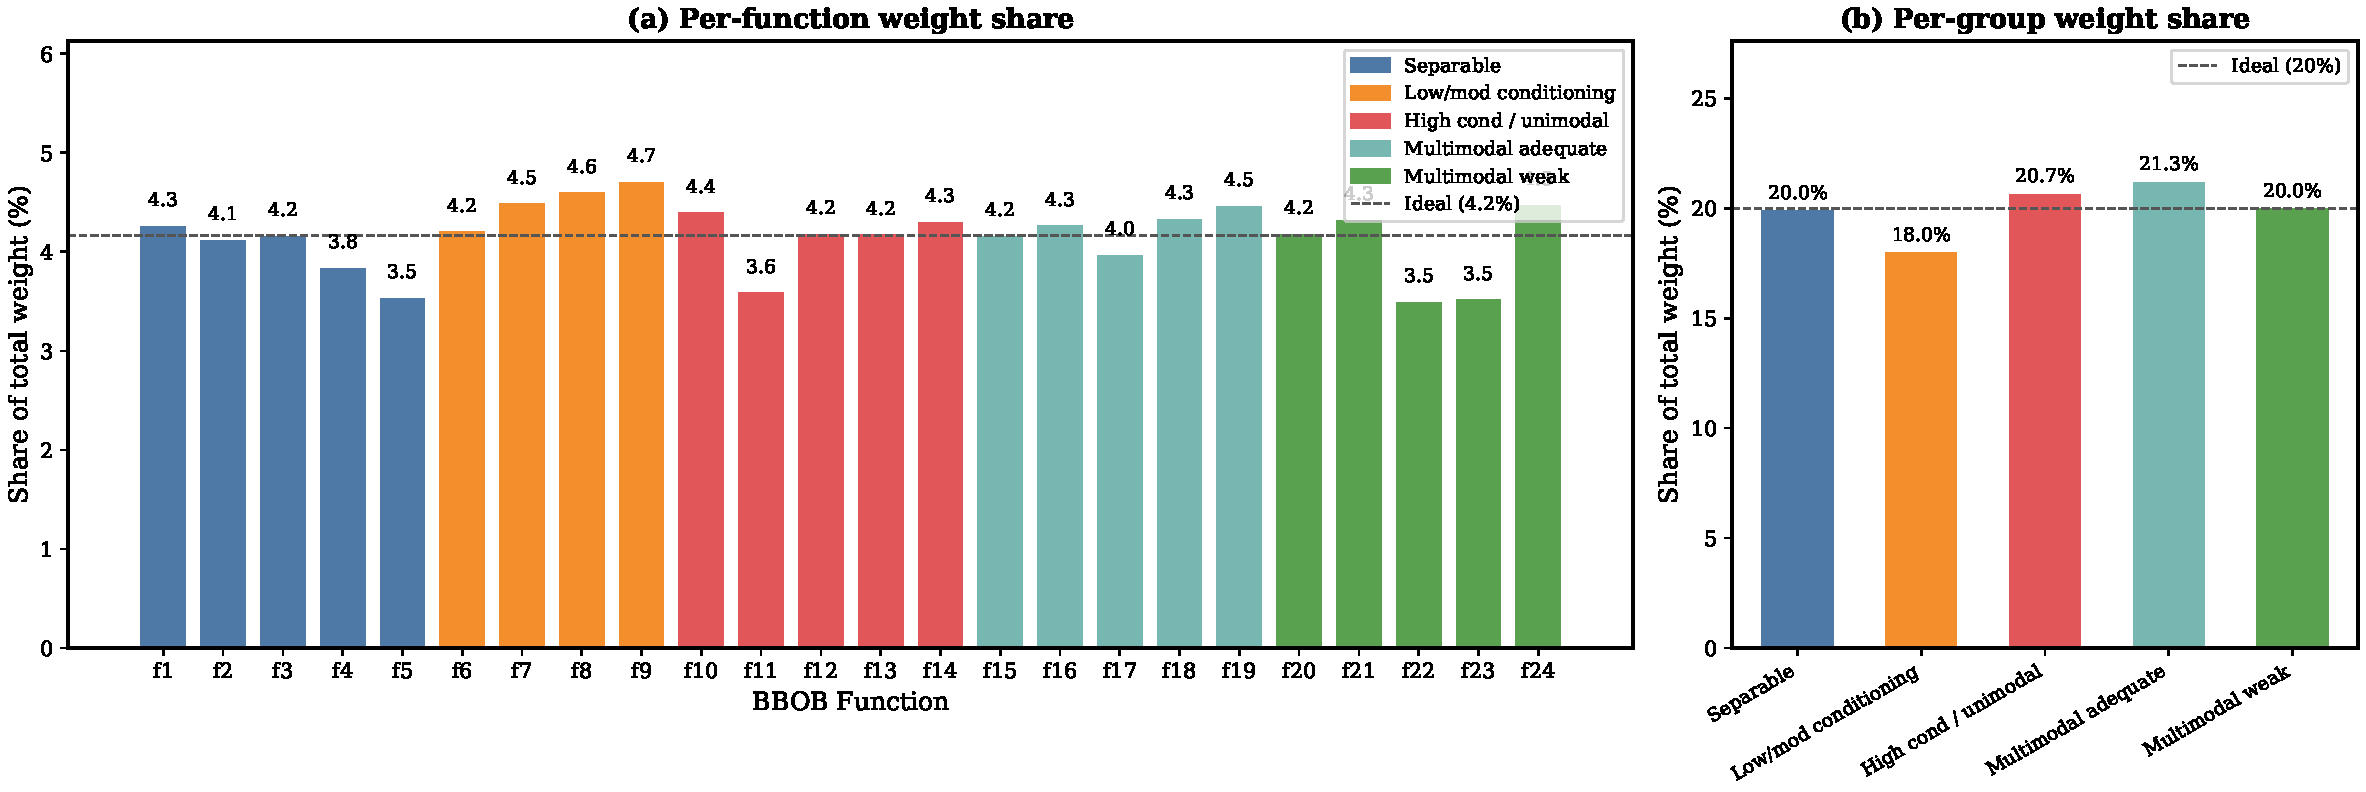
\includegraphics[width=\textwidth]{figures/fig_mabbob_instances_phase4.pdf}
  \caption{Per-BBOB-function (left) and per-group (right) weight distribution of the 20 MA-BBOB functions used in Stage~4. Dashed lines mark the ideal uniform shares (4.2\% per BBOB function, 20\% per group). All 24 BBOB functions are covered, with a coefficient of variation of $0.080$ across per-BBOB-function totals and group shares within $\pm$1.3\% of the ideal.}
  \label{fig:mabbob-instances-phase4}
\end{figure*}

\begin{table*}[!t]
\centering
\caption{BBOB function weights for the 20 MA-BBOB functions used in Stage~4. Values are percentages of total weight; empty cells indicate zero weight.}
\label{tab:instance-weights-phase4}
\scriptsize
\begin{tabular}{@{}r|cccccccccccccccccccccccc@{}}
\toprule
\textbf{Func.} & \textbf{1} & \textbf{2} & \textbf{3} & \textbf{4} & \textbf{5} & \textbf{6} & \textbf{7} & \textbf{8} & \textbf{9} & \textbf{10} & \textbf{11} & \textbf{12} & \textbf{13} & \textbf{14} & \textbf{15} & \textbf{16} & \textbf{17} & \textbf{18} & \textbf{19} & \textbf{20} & \textbf{21} & \textbf{22} & \textbf{23} & \textbf{24} \\
\midrule
22  &    & 18 &    &    & 7  & 13 &    &    & 18 &    &    & 15 & 3  &    &    &    &    &    & 12 &    &    & 13 &    &    \\
93  &    &    &    &    &    &    &    &    & 19 &    & 16 &    & 23 &    &    &    &    & 18 & 20 &    &    &    & 4  &    \\
166 &    &    &    &    &    &    &    &    &    &    &    &    &    & 15 & 17 &    &    & 23 &    & 30 &    &    &    & 15 \\
196 & 5  & 19 &    &    & 11 & 10 &    &    &    &    &    &    &    &    & 15 & 11 &    & 4  &    &    & 10 &    &    & 16 \\
203 &    & 30 &    &    & 30 & 18 &    &    &    &    & 22 &    &    &    &    &    &    &    &    &    &    &    &    &    \\
288 &    &    &    & 23 &    &    & 7  &    &    & 27 & 7  &    &    &    &    &    &    &    &    &    & 29 &    & 7  &    \\
321 &    &    &    & 9  &    & 5  & 16 &    & 17 & 10 &    & 18 & 8  &    &    &    & 5  & 12 &    &    &    &    &    &    \\
408 & 24 &    &    & 14 &    &    &    &    &    &    &    &    &    &    &    &    &    & 19 & 20 &    & 22 &    &    &    \\
480 & 19 &    & 22 & 3  &    &    & 6  &    &    &    &    &    &    &    & 8  & 13 &    &    & 10 &    & 18 &    &    &    \\
513 & 15 &    & 27 &    &    &    &    &    &    &    &    &    &    &    &    & 18 &    &    &    & 14 &    &    &    & 26 \\
528 &    &    & 22 &    & 18 &    & 11 &    &    & 3  &    & 12 & 22 &    &    & 10 &    &    &    &    & 1  &    &    &    \\
598 &    &    &    &    &    &    &    & 29 &    &    &    &    &    & 30 &    &    & 27 &    &    & 2  &    &    & 12 &    \\
697 &    &    &    &    &    &    &    & 3  &    & 32 &    & 4  &    & 27 &    & 7  &    &    &    &    & 6  &    & 21 &    \\
781 &    & 15 &    &    &    &    &    &    & 14 &    & 12 &    &    &    &    & 13 & 21 & 10 &    & 15 &    &    &    &    \\
784 &    &    & 12 &    & 5  &    & 12 &    &    &    & 15 & 24 &    &    & 19 &    &    &    &    &    &    & 12 &    &    \\
803 &    &    &    &    &    &    & 21 & 19 &    &    &    &    & 21 &    & 15 & 13 &    &    & 7  & 5  &    &    &    &    \\
894 & 14 &    &    &    &    & 14 &    &    & 16 & 16 &    &    & 6  &    & 10 &    &    &    & 21 &    &    &    &    & 3  \\
947 & 3  &    &    &    &    & 12 & 17 & 18 & 10 &    &    &    &    &    &    &    & 5  &    &    & 17 &    &    &    & 18 \\
951 & 5  &    &    & 3  &    & 12 &    & 11 &    &    &    &    &    &    &    &    & 22 &    &    &    &    & 20 & 27 &    \\
999 &    &    &    & 24 &    &    &    & 13 &    &    &    & 11 &    & 15 &    &    &    & 1  &    &    &    & 25 &    & 12 \\
\bottomrule
\end{tabular}
\end{table*}

